\documentclass{article}
% \usepackage[utf8]{inputenc}
\usepackage[backend=biber,citestyle=ieee]{biblatex}

\usepackage{pgfgantt}
\usepackage{graphicx}
\usepackage{xcolor}
\usepackage{float}
\usepackage{subfig}
\usepackage{listings}

\definecolor{codegreen}{rgb}{0,0.6,0}
\definecolor{codegray}{rgb}{0.5,0.5,0.5}
\definecolor{codepurple}{rgb}{0.58,0,0.82}
\definecolor{backcolour}{rgb}{0.95,0.95,0.95}

\lstdefinestyle{mystyle}{
    backgroundcolor=\color{backcolour},   
    commentstyle=\color{codegreen},
    keywordstyle=\color{magenta},
    numberstyle=\tiny\color{codegray},
    stringstyle=\color{codepurple},
    basicstyle=\ttfamily\footnotesize,
    breakatwhitespace=false,         
    breaklines=true,                 
    captionpos=b,                    
    keepspaces=false,                 
    numbers=left,                    
    numbersep=5pt,                  
    showspaces=false,                
    showstringspaces=false,
    showtabs=false,                  
    tabsize=1
}

\lstset{style=mystyle}


% \usepackage{a4wide} 

\usepackage{fancyhdr}   %sidhuvud
\pagestyle{fancy}

\addbibresource{sources.bib}

\newcommand{\getauthor}{Oscar Fredriksson} %Author
\newcommand{\gettitle}{NS3 - Lab} %Title

\title{\gettitle}
\author{\getauthor}
\date{April 2021}

\begin{document}

    \pagenumbering{gobble}
    \maketitle

    \newpage

    \pagenumbering{arabic}

    \fancyhf{}
    \lhead{\getauthor}
    \rhead{\gettitle}
    \rfoot \thepage

    \section{Startup}

    \subsubsection*{What is the network topology?}
    The simulated network topology is a simple point to point connection, a diagram of the topology can be seen in figure \ref{fig:topology}.

    \begin{figure}[H]
        \centering
        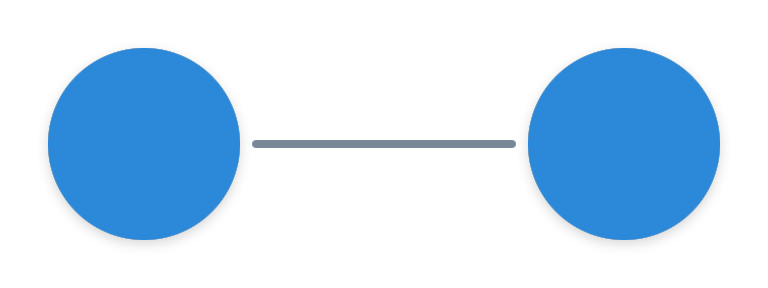
\includegraphics[width=0.5\textwidth]{img/topology.png}
        
        \caption{The simulated topology, a simple point to point connection.}
        \label{fig:topology}
    \end{figure}

    \subsubsection*{How many queues are used in each node? How are they configured?}
    The system uses two different queues, a \verb|FifoQueueDisc| that can hold a specific number of packets configured by the parameter \verb|queueSize| and a \verb|DropTailQueue| that can hold a single packet and drops any overflow. The \verb|FifoQueueDisc| feeds into the \verb|DropTailQueue| which means a total queue size of \verb|queueSize+1| with any extra packets on route to each node gets dropped by the \verb|DropTailQueue|. 

    \subsubsection*{Does the channel introduce errors?}
    The channel does not introduce errors. 

    \subsubsection*{What are the configuration variables of the code?}
    The configuration variables of the code are the arrival rate, \verb|lambda|, the service rate, mu, aswell as \verb|queueSize| and \verb|simulationTime|.

    \subsubsection*{What output files are generated?}
    Two files are generated, one for each node, with captured packets. The files are called \verb|ms-lab7-0-0.pcap| and \verb|ms-lab7-1-0.pcap|. The captured packets in the files can be inspected using wireshark.

    \section{Simulation}

    \subsubsection*{What values should the configuration variables (program arguments) of the code?}
    The arrival rate ($\lambda$) and service rate ($\mu$) variables are set to the given values in the task, where the sensor data generation rate is the arrival rate and the interface send out rate the service rate. To simulate an "almost infinite" buffer the \verb|queueSize| parameter was set to 100 000, the \verb|simulationTime| simply needs to be set to an adequetely large value to simulate long enough to see the behaviour, it was set to 500. The values of the configured parameters can be seen in table \ref{tab:parameters}.

    \begin{table}[H]
        
        \begin{center}
        \begin{tabular}{ |c|c| } 
            \hline
        Parameter & Value \\\hline\hline
            $\lambda$ & 300 \\\hline 
            $\mu$ & 330 \\\hline
            queueSize & 100 000 \\\hline 
            simulationTime & 500 \\\hline
        \end{tabular}
        \end{center}
    \caption{The configuration parameters set for the simulation.}
    \label{tab:parameters}
    \end{table}

    \subsubsection*{How will you calculate the average buffer size?}
    After removing the warm-up period by removing leading zeros in the \verb|queue-1.tr| file the average number of packets in the queue can be calculated by taking the average of the rest of the measurements in the file. The average number of packets in the buffer was found to be $\approx7.8$ packets, which can be rounded up to give as an average buffer size of 8.

    \subsubsection*{How long should the simulation last?}
    The simulation should run long enough to get well past the warm-up period and get enough readings to calculate a reliable average. 

    \subsubsection*{What value of warm-up time will you use?}
    A warmup time value of 35 (removing the first 35 rows in \verb|queue-1.tr|) will be used.

    \subsubsection*{How many independent simulation runs have you performed?}
    4 independent simulation runs was done to make sure the results doesn't differ to much between runs.

    \subsubsection*{Compare your findings to the mathematical model}
    The packet loss of the "infinite" buffer size of 100 thousand packets is unsurprisingly 0\%. The theoretical packet loss of a buffer of size $K$ can be calculated using equation \ref{eqn:theoretical-packet-loss} 
    
    \begin{equation}
    \label{eqn:theoretical-packet-loss}
        P_K = \rho^K\frac{1-\rho}{1-\rho^{K+1}}
    \end{equation}
    
    By applying this formula to the buffer size of 100 thousand packets we can see that, just like the simulations, this has a theoretical packet loss of 0\%, which can be seen in equation \ref{eqn:100k-buffer-size}.

    \begin{equation}
    \label{eqn:100k-buffer-size}
        P_{100000} = \left(\frac{300}{330}\right)^{100000}\frac{1-(\frac{300}{330})}{1-(\frac{300}{330})^{100001}} = 0 
    \end{equation}

    \subsubsection*{Simulate the case with a limited buffer and find the packet loss probability}
    The same simulation was run with a buffer size of 8 (by setting the \verb|queueSize| variable to 8) and the following output was achieved.

    \begin{lstlisting}
        *** Flow monitor statistics ***
        Tx Packets/Bytes: 149879 / 56265782
        Offered Load: 0.902064 Mbps
        Rx Packets/Bytes: 142452 / 53216806
        Packets/Bytes Dropped by Queue Disc: 7518 / 3223778
        Packets/Bytes Dropped by NetDevice: 0 / 0
        Throughput: 0.853187 Mbps
    \end{lstlisting}

    By reading the number of dropped packets on row 5 and the total number of sent packets on row 2 we can calculate the packet loss using equation \ref{eqn:packet-loss-test}.

    \begin{equation}
    \label{eqn:packet-loss-test}
        \frac{7518}{149879} = 0,0502 = 5.02\% 
    \end{equation}

    \subsubsection*{Compare your findings to the mathematical model}

    The formula for theoretically estimating the packet loss has been stated earlier in equation \ref{eqn:theoretical-packet-loss}, applying this to the buffer size of 8, we get 7.36\% as can be seen in equation \ref{eqn:8-buffer-size}.

    \begin{equation}
    \label{eqn:8-buffer-size}
        P_{8} = \left(\frac{300}{330}\right)^{8}\frac{1-(\frac{300}{330})}{1-(\frac{300}{330})^{9}} = 0,0736 = 7.36\%
    \end{equation}

    \subsubsection*{How large should the buffer be so that the loss is no greater than 1\%? Can you easily calculate this from the methematical model?}

    Using trial and error by tweaking the buffer size a buffer of size 25 was found to have a packet loss of 0.65\%. The theoretical buffer size to have less than a 1\% packet loss can be found by solving equation \ref{eqn:1percent-buffer}.

    \begin{equation}
    \label{eqn:1percent-buffer}
        0.01 = \rho^K\frac{1-\rho}{1-\rho^{K+1}}
    \end{equation}

    Using an online equation solver tool \cite{wolfram} $K$ was found to be $\approx24.1589$, which gets rounded up to a buffer size of 25 to get less than 1\%.

    \subsubsection*{Modify the simulation to have a M/D/1 queue, compare the results with the mathematical expression.}
    To simulate a M/D/1 queue the code was modified to generate packets constant size, which in turn gives us a constant service rate with no variation. The modified code can be seen below. 

    \begin{lstlisting}[language=C]
    static void GenerateTrafficMD1(Ptr<Socket> socket, Ptr<ExponentialRandomVariable> randomTime, double mu) 
    {
        const uint32_t size = (1000000.0/(8*mu)-30);
        socket->Send(Create<Packet> (size));
    
        Time pktInterval = Seconds(randomTime->GetValue());
        Simulator::Schedule(pktInterval, &GenerateTrafficMD1, socket, randomTime, mu);
    }
    ...    

    Simulator::ScheduleWithContext(source->GetNode()->GetId(), Seconds(1.0), &GenerateTrafficMD1, source, randomTime, mu);
    \end{lstlisting}

    Running this modified code with all the same parameters as the previous simulation the average queue size was $\approx3.76$. The mathematical theoretical value for the average queue size was calculated to $\approx4.55$ as can be seen in equation \ref{eqn:md1-avg-queue}.

    \begin{equation}
    \label{eqn:md1-avg-queue}
        N_q = \frac{\lambda^2*\frac{1}{\mu^2}}{2(1-\rho)} = \frac{300^2*\frac{1}{330^2}}{2\left(1-\frac{300}{330}\right)} = 4.55
    \end{equation}

    

    \newpage
    \printbibliography

\end{document}